\question Escribe el grupo, período y clasificación de los siguientes elementos. Después de realizar este ejercicio, ubica a cada elemento en la tabla
periódica que se muestra abajo.


\begin{tabular}{c|c|c|c}
    \hline
                            & grupo & período & familia \\ \hline
    Polonio                 &       &         &         \\    \hline
    Manganeso               &       &         &         \\    \hline
    Magnesio                &       &         &         \\    \hline
    Xenón                   &       &         &         \\    \hline
    Ión negativo de Oxígeno &       &         &         \\    \hline
    Silicio                 &       &         &         \\    \hline
    Ión positivo de Calcio  &       &         &         \\    \hline
    Criptón                 &       &         &         \\    \hline
    Ión positivo de Litio   &       &         &         \\    \hline
    Fósforo                 &       &         &         \\    \hline
    Selenio                 &       &         &         \\    \hline
    Ión positivo de Sodio   &       &         &         \\    \hline
    Ión negativo de Cloro   &       &         &         \\    \hline
    Nitrógeno               &       &         &         \\    \hline
    Ión positivo de Silicio &       &         &         \\    \hline
    Neón                    &       &         &         \\    \hline
    Bromo                   &       &         &         \\    \hline
    Calcio                  &       &         &         \\    \hline
    Oro                     &       &         &         \\    \hline
    Ión negativo de Fluor   &       &         &         \\    \hline
    Rubidio                 &       &         &         \\    \hline
    Hidrógeno               &       &         &         \\    \hline
    Carbono                 &       &         &         \\    \hline
\end{tabular}

\begin{figure}[H]
    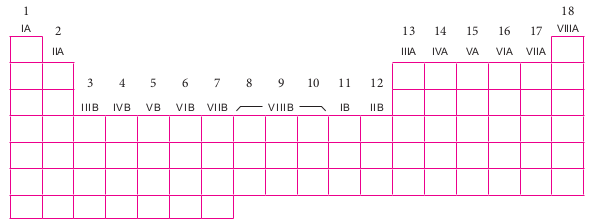
\includegraphics[width=\linewidth]{../images/tablavacia.png}
\end{figure}